\section{Introducción}
La seguridad ciudadana es uno de los problemas principales de las sociedades en varios países de América Latina, es por ello que sus habitantes viven preocupados por el constante aumento en la tasa de criminalidad. Estos se sienten cada vez más inseguros en sus personas y bienes, y denotan su insatisfacción con respecto a las respuestas estatales ante el fenómeno delictivo\cite{rico2002seguridad}.

Este fenómeno es un tema complejo, y muchas veces cualquier acción que se realice para prevenirlo o controlarlo aparenta insuficiente. Para ello es fundamental desarrollar diagnósticos de calidad basados en indicadores válidos y confiables.

En Paraguay, en fecha 18 de octubre de 2012, fue sancionada la Ley que crea el Sistema Nacional de Emergencias denominado 911, para la atención de comunicaciones de emergencias. El sistema 911 funciona en un moderno centro de comando y recibe aproximadamente 7 mil llamadas diarias\cite{ensc2014}. Para optimizar la función del Sistema de Emergencia Policial 911, la Policía Nacional dispuso que las comisarías cumplan funciones de emergencia.

Las llamadas dirigidas al 911 pasan por 4 etapas de tiempos (figura \ref{fig:time1}), que están definidas como (1) recepción, (2) procesamiento, (3) asignación del recurso policial encargado y (4) desplazamiento del recurso asignado.

\begin{figure}[!ht]
    \centering
    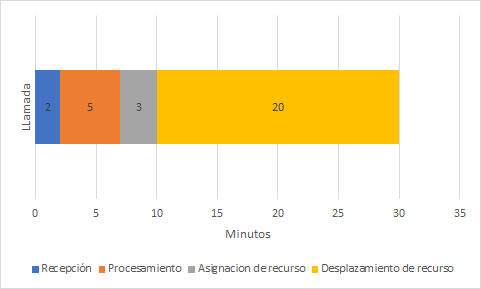
\includegraphics[width=88mm,scale=0.5]{images/tiempo_llamadas.png}
    \caption{Tiempo de vida promedio por llamada.}
    \label{fig:time1}
\end{figure}

A partir de lo citado anteriormente, se tomó como referencia el trabajo \textit{``A Tabu Search based heuristic for police units positioning''}\cite{7359471} para obtener posiciones óptimas en la ubicación de los recursos policiales utilizando el procedimiento meta-heurístico de la búsqueda Tabú. A fin de obtener valores más precisos fueron necesarios aplicar modificaciones al trabajo referenciado.

Este trabajo, se enfoca en la optimización de la etapa 4 (desplazamiento del recurso) de las llamadas (figura \ref{fig:time1}), de tal forma a reducir al mínimo posible el tiempo transcurrido desde el inicio de la llamada hasta la asistencia del recurso policial, mediante la utilización del histórico de datos delictivos con georeferencias.